\subsection{Avancées et prévisions}
\subsubsection{Avancées}
\begin{table}[!hbt]
    \begin{center}
        \begin{tabular}{l|ll}
            \rowcolor[HTML]{000000} 
            {\color[HTML]{FFFFFF} \backslashbox{\textbf{Partie}}{\textbf{Tâche}}} & {\color[HTML]{FFFFFF} \textbf{Prévu}} & {\color[HTML]{FFFFFF} \textbf{Réalisé}} \\
            \rowcolor[HTML]{FFFFFF} 
            \textbf{Mouvement}                         & 70\%                                  & \cellcolor[HTML]{68CBD0}70\%         \\
            \rowcolor[HTML]{C0C0C0} 
            \textbf{Interface/HUD}                     & 60\%                                  & \cellcolor[HTML]{FD6864}50\%         \\
            \textbf{Cartes}                            & 80\%                                  & \cellcolor[HTML]{68CBD0}90\%         \\
            \rowcolor[HTML]{C0C0C0}
			\textbf{Réseau}    						   & 50\%          						   & \cellcolor[HTML]{FFCC67}70\%         \\
            \textbf{IA}                                & 60\%                                  & \cellcolor[HTML]{FFCC67}80\%         \\
            \rowcolor[HTML]{C0C0C0} 
            \textbf{Mécaniques de jeu}                 & 70\%                                  & \cellcolor[HTML]{FFCC67}80\%         \\
            \textbf{Progression}                       & 60\%                                  & \cellcolor[HTML]{FD6864}50\%        
            \end{tabular}
    \end{center}
    \caption{Tableau des avances et retards dans les différentes parties}
\end{table}
	\subsubsection{Prévisions}
	Le jeu est à présent dans un état "jouable". Cependant, il faut encore implémenter de nombreux systèmes pour finaliser notre vision pour le projet.

	\subsubsection{Multiplayer}
	Certains systèmes ont été créés, comme les finishers ou les pouvoirs, mais n'ont pas encore été 
	implémentés en multijoueur. L'objectif pour la prochaine soutenance sera donc d'intégrer les mécaniques 
	de jeu qui ne l'ont pas encore été au réseau Photon pour permettre au joueurs d'y accéder. De plus, le 
	travail continue sur la synchronisation ie. des personnages joueurs et non-joueurs, notamment il est 
	question d'optimisation pour le mouvement des IA qui génère encore une utilisation de bande passante importante. 
	Il serait intéressant de tenter l'utilisation d'une méthode de compression pour les vecteurs afin de diminuer 
	la quantité d'information envoyée.

	\subsubsection{Progression}
		Bien qu'un système d' expérience et de niveau ait été implémenté, celui-ci n'a pour l'instant pour 
		l'instant pas d'utilité. Mais de nombreuses opportunités de progression se sont ouvertes, 
		notamment grâce au travail de Dov. Par exemple, nous comptons permettre le débloquage des 
		finishers grâce à ce système de progression. Nous pourrons également modifier le système actuel 
		de customisation de personnage et restreindre l'utilisation de certaines options d'apparence à un certain niveau.

    \subsubsection{Tableau des scores}
    Le scoreboard reste très simple et manque d’informations. Nous souhaiterions donner au tableau des scores un affichage plus épuré et plus simple. Une mise en tableau des différentes informations permettrait d’éviter au texte de dépasser les bordures du canvas. Elle facilitera grandement l’ajout, la suppression ou la modification d’une valeur ou d’un joueur pendant la partie ainsi que l’alignement des valeurs appartenant a la même categorie. 
    Cette nouvelle version du tableau comprendrai l'affichage des points, du nombre de fois où le joueur est mort, le nombre de fois où il a tué un joueur, le nombre de fois ou il a tué une IA et son PING avec le serveur.
    Ce formatage sous forme de tabeau permet aussi de faire une sauvegarde rapide et temporaire du tableau dans les fichiers du jeu. Il serait ainsi beaucoup plus simple pour le logiciel d'y acceder et de l'editer.
    
    \begin{figure}[hbt!]
            \centering
            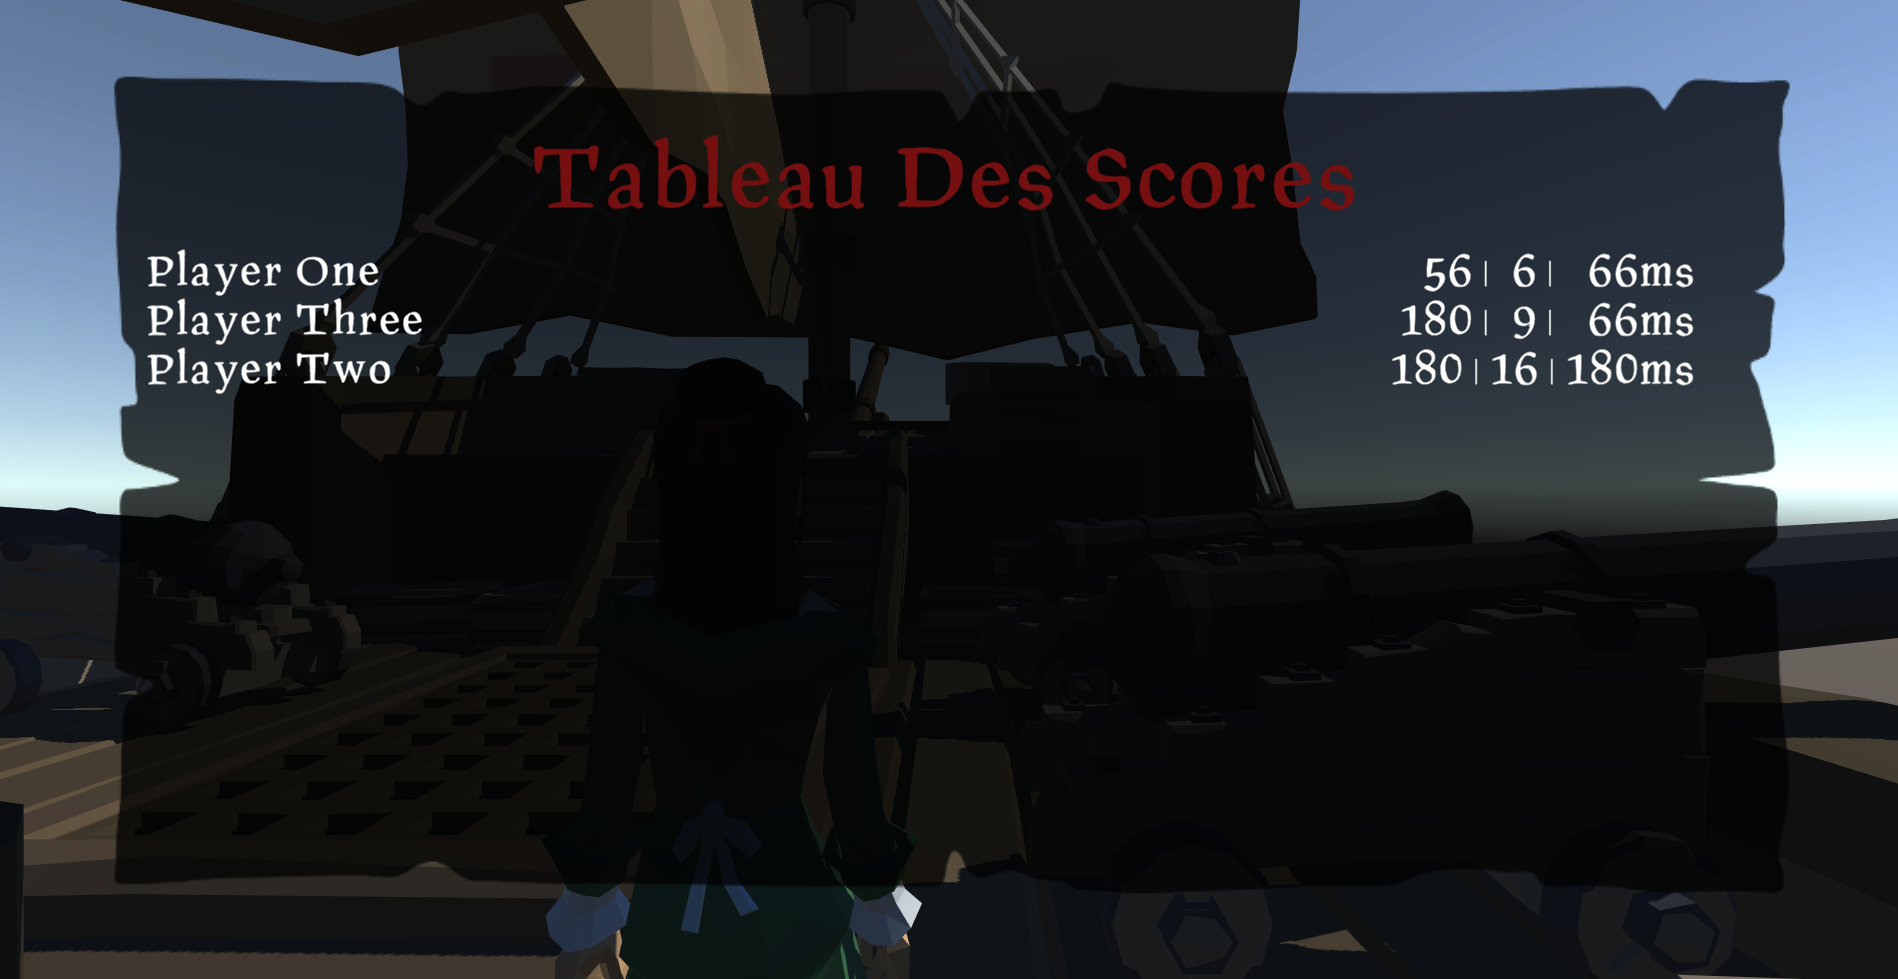
\includegraphics[scale=0.3]{img/newscoreboard.PNG}
            \caption{Seconde version du tableau des scores}
    \end{figure}


    \subsubsection{HUD}
    

	\subsubsection{Carte}

	Pour la prochaine soutenance, l'objectif est d'avoir une map terminée dans les moindres 
	détails. Comme cet objectif semble raisonnable, un seconde carte est aussi une possibilité 
	envisagée pour l'ultime soutenance.